% =====================================================================
%  §0. Электродинамика: необходимый минимум
%  Источник фактуры: BRIEF_FOR_D_teaching_ladder.md §2 (модуль 00)
%  Markdown-версия: research/paper/primers/00_electrodynamics_minimum.md
% =====================================================================
\section{Электродинамика: необходимый минимум}
\label{sec:electrodynamics}
\markboth{§\thesection. Электродинамика: необходимый минимум}{}

Этот параграф отвечает на четыре вопроса, которые дальше принимаются молча: почему волна
описывается \emph{комплексным} числом; почему терагерцовый прибор меряет \emph{поле}, а не
привычную интенсивность; почему решётка проводов ведёт себя как \emph{сплошной} анизотропный лист;
и почему вся геометрия образца сворачивается в \emph{одно} безразмерное число.

\begin{tcolorbox}[enhanced,colback=cPanel,colframe=cGrid,boxrule=0.8pt,arc=2pt,
                  title={\bfseries\color{cAccent} Пререквизиты},coltitle=cAccent,
                  attach boxed title to top left={xshift=6pt,yshift=-2pt},
                  boxed title style={colback=cPanel,boxrule=0pt,arc=0pt},top=10pt]
\textbf{Нужно знать:} что такое частота, длина волны и период; связь $\lambda=c/\nu$; комплексные
числа (модуль, аргумент, формула Эйлера $e^{\jj\varphi}=\cos\varphi+\jj\sin\varphi$); проекции
вектора на оси.\\[0.3em]
\textbf{Знать НЕ нужно:} уравнения Максвелла, тензорный анализ, теорию дифракции. Ни одно из этого
здесь не потребуется. Всё, что не используется в последующих параграфах, опущено сознательно.
\end{tcolorbox}

% ---------------------------------------------------------------------
\subsection{Плоская волна и комплексная амплитуда}

\begin{intuition}
Электромагнитная волна~--- колебание электрического поля, бегущее в пространстве. В точке детектора
поле есть просто функция времени: синусоида с некоторой амплитудой (насколько сильно) и фазой
(в какой момент максимум).
\end{intuition}

\noindent
Монохроматическая плоская волна, бегущая вдоль оси~$z$, записывается как
\[
  E(z,t)=A\cos(\omega t-kz+\varphi_0),
  \qquad \omega=2\pi\nu,\qquad k=\frac{2\pi}{\lambda}=\frac{\omega}{c},
\]
где $A$~--- \term{амплитуда}, $\varphi_0$~--- \term{начальная фаза}, $k$~--- \term{волновое число}.

\paragraph{Зачем нужна комплексная запись.} С косинусами работать неудобно: при прохождении через
оптический элемент амплитуда \emph{умножается}, а фаза \emph{сдвигается}~--- две разные операции.
Комплексная запись сводит их к одному умножению:
\[
  E(z,t)=\Real\!\left[\Efield\,e^{\jj(\omega t-kz)}\right],
  \qquad \Efield=A\,e^{\jj\varphi_0}.
\]
Число $\Efield$~--- \term{комплексная амплитуда}: её модуль $|\Efield|=A$ хранит «насколько
сильно», её аргумент $\arg\Efield=\varphi_0$ хранит «когда». Оптический элемент с пропусканием
$t=|t|e^{\jj\delta}$ действует как $\Efield\mapsto t\,\Efield$: модули перемножились, фазы
сложились. Одно умножение вместо тригонометрии.

\begin{strict}[: что отсюда растёт]
Величины $\tperp$ и $\tpar$~--- пропускание решётки для двух поляризаций (см.
\S\ref{subsec:grid})~--- суть именно комплексные числа. Каждое из них есть \emph{два} вещественных
числа на каждой частоте: сколько прошло и с какой задержкой.
\end{strict}

% ---------------------------------------------------------------------
\subsection{Фаза~--- не бухгалтерия, а измеряемая физика}
\label{subsec:phase}

Соблазн неспециалиста~--- считать фазу технической деталью, а «настоящий» результат видеть в
амплитуде. В этом проекте фаза несёт самостоятельный физический результат.

\begin{strict}[: наклон фазы есть время]
Если фаза линейно зависит от частоты, $\delta(\nu)=\delta_0+2\pi\nu\tau$, то $\tau$~---
\term{временная задержка} сигнала. Проверяется прямой подстановкой в выражение предыдущего
раздела: такая фаза даёт $E(t)\mapsto E(t-\tau)$. Значит, \emph{наклон фазы по частоте измеряет
время}.
\end{strict}

\begin{projectfact}[: задержка утечки, измеренная двумя способами]
У утечки тёмного канала обнаружена собственная групповая задержка
\[
  \tleak\approx0.19\ \text{пс}
  \qquad\text{(гипотеза HN8; } \dAIC=-579 \text{ поверх HN2).}
\]
Независимое подтверждение~--- \emph{прямой сдвиг пика импульса во времени на $-0.31$~пс}.
\artifact{research/SYNTHESIS.md} (линия HN8);
сводка~--- \artifact{research/two\_wgp/BRIEF\_FOR\_D\_teaching\_ladder.md} §7.1.

Величина, извлечённая из наклона фазы в частотной области, видна невооружённым глазом во временной.
\end{projectfact}

\begin{intuition}[: почему это убедительно]
Два способа получить одно число используют разные части данных и разные предположения. Совпадение~---
не арифметическая проверка, а физический аргумент: задержка реальна, а не является артефактом
модели. Этот приём («триангуляция») разбирается в~\S10.
\end{intuition}

% ---------------------------------------------------------------------
\subsection{Поле или интенсивность~--- ключевое различие}
\label{subsec:field-vs-intensity}

\begin{intuition}
Обыденная оптическая интуиция построена на \emph{интенсивности}. Глаз, фотодиод, болометр,
ПЗС-матрица меряют мощность~$\propto|E|^2$, усреднённую по многим периодам колебания. Фаза при
этом теряется безвозвратно. Терагерцовый прибор устроен принципиально иначе.
\end{intuition}

\noindent
\term{THz-TDS} (терагерцовая спектроскопия во временной области) выполняет \term{когерентное
стробирование}: фемтосекундный импульс лазера открывает детектор на мгновение, много более
короткое, чем период терагерцового колебания, и прибор записывает \emph{мгновенное значение поля}
$E(t)$, а не его квадрат. Данные проекта устроены именно так~--- две колонки, время и поле
\artifact{data\_pool/\{dataset\}\_\{angle\}deg\_rep\{N\}\_\{sig|bg\}.txt}.

\paragraph{Следствие, определяющее всю математику проекта.} Пусть поле на детекторе есть сумма
двух каналов (вывод~--- \S1):
\begin{equation}
  \Efield(\theta)=\tperp\cos^2\theta+\tpar\sin^2\theta .
  \label{eq:two-channels}
\end{equation}
Энергетическая наблюдаемая $U=|\Efield|^2$ тогда содержит \term{перекрёстный член}:
\begin{equation}
  U(\theta)=|\tperp|^2\cos^4\theta+|\tpar|^2\sin^4\theta
  +2\,\Real\!\left(\tperp\overline{\tpar}\right)\cos^2\theta\sin^2\theta .
  \label{eq:U-cross}
\end{equation}

\begin{warning}[: третье слагаемое существует не всегда]
Перекрёстный член в~\eqref{eq:U-cross} возникает \emph{только потому, что каналы когерентны}~---
то есть складываются поля, а не мощности. Если бы прибор мерил интенсивности, слагаемого не было бы,
и вместе с ним исчезла бы вся информация об относительной фазе каналов, то есть о~$\tleak$.
\end{warning}

\begin{figure}[t]
  \centering
  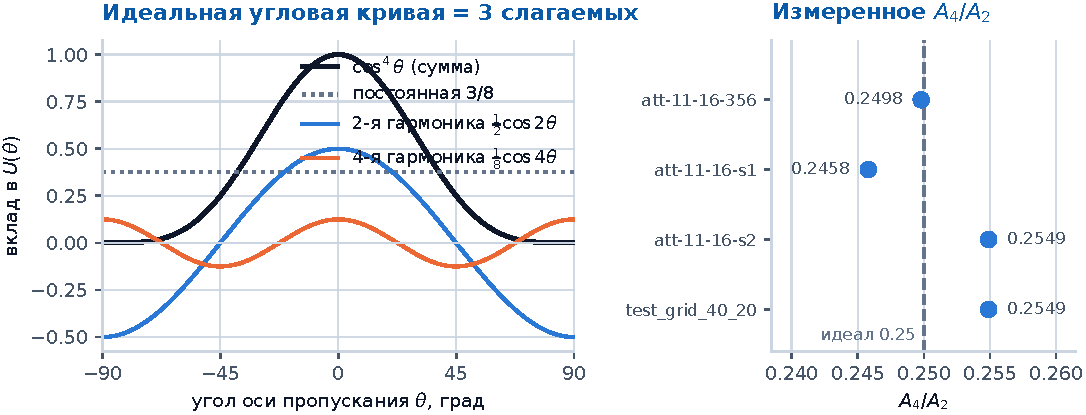
\includegraphics[width=\linewidth]{figures/fig00_harmonics.pdf}
  \caption{Слева: идеальная угловая кривая $\cos^4\theta$ раскладывается ровно на постоянную,
  вторую и четвёртую гармоники угла~--- это тождество, а не приближение. Справа: измеренное
  отношение амплитуд четвёртой и второй гармоник против идеального значения~$0.25$; отклонение
  менее~2\,\%. Числа перенесены из \artifact{BRIEF\_FOR\_D\_teaching\_ladder.md} §5.2.}
  \label{fig:harmonics}
\end{figure}

\paragraph{Цена вопроса~--- конкретное число.} Из-за перекрёстного члена угловая зависимость
$U(\theta)$ раскладывается по \emph{пяти} функциям
$\{1,\cos2\theta,\sin2\theta,\cos4\theta,\sin4\theta\}$, а не по трём, как было бы в некогерентном
(учебном) случае. Именно четвёртая гармоника несёт относительную фазу каналов, то есть~$\tleak$
из~\S\ref{subsec:phase}.

\begin{projectfact}[: разложение точно, а не приближённо]
Численная проверка на синтетике: невязка разложения $\mathrm{rms}=1.4\times10^{-16}$~--- машинный
ноль. \artifact{research/two\_wgp/NOTE\_malus\_linearization.md}, артефакт
\artifact{research/results/two\_wgp/a0\_malus\_linearization.json}.

Отношение амплитуд четвёртой и второй гармоник для идеального $\cos^4\theta$ равно ровно~$0.25$;
на данных~--- \texttt{356att} $0.2498$, \texttt{s1} $0.2458$, \texttt{s2} $0.2549$,
\texttt{test\_grid} $0.2549$ (рис.~\ref{fig:harmonics}). Игнорировать четвёртую гармонику~---
значит выбросить около четверти сигнала.
\end{projectfact}

\begin{tcolorbox}[enhanced,colback=cS1!7,colframe=cS1,boxrule=0pt,leftrule=3pt,arc=1pt]
\textbf{Мораль для всего курса.} Различение «поле против интенсивности»~--- не философия. Оно
решает, сколько независимых чисел содержит одно измерение: \textbf{пять, а не три}. А сколько чисел
содержит измерение~--- это, как выяснится в~\S5 и~\S9, и есть главный вопрос всего проекта:
параметров в модели может быть больше, чем измерение содержит независимых чисел.
\end{tcolorbox}

% ---------------------------------------------------------------------
\subsection{Поляризация и поворот осей}

\begin{intuition}
Волна бежит вдоль~$z$, поле колеблется поперёк~--- в плоскости $(x,y)$. \term{Поляризация} отвечает
на вопрос, по какой траектории в этой плоскости движется кончик вектора поля. Вдоль прямой~---
\emph{линейная} поляризация, и её достаточно задать одним углом.
\end{intuition}

\noindent
Поле под углом~$\alpha$ к оси~$x$ раскладывается на проекции, а переход между системами координат
выполняется обычной матрицей поворота:
\[
  \vec{E}=E_0\begin{pmatrix}\cos\alpha\\ \sin\alpha\end{pmatrix},
  \qquad
  \Rot{\theta}=\begin{pmatrix}\cos\theta & -\sin\theta\\[2pt] \sin\theta & \cos\theta\end{pmatrix}.
\]
Этого достаточно: физика элемента записывается в его \emph{собственных} осях, а в лабораторные
переводится сопряжением $\Rot{\theta}\,(\cdot)\,\Rot{-\theta}$. Подробный разбор с выводом закона
Малюса~--- \S1.

% ---------------------------------------------------------------------
\subsection{Решётка проводов как анизотропный лист}
\label{subsec:grid}

\begin{intuition}
Проволочный поляризатор~--- плоскость параллельных металлических проволок. Что произойдёт с волной,
зависит только от ориентации поля относительно проволок. Поле \emph{вдоль} проволок гонит электроны
вдоль проволоки, течёт ток, ток переизлучает волну назад~--- волна отражается. Поле \emph{поперёк}
проволок двигать электроны почти не может (поперёк проволока тонкая)~--- волна проходит.
\end{intuition}

\begin{figure}[t]
  \centering
  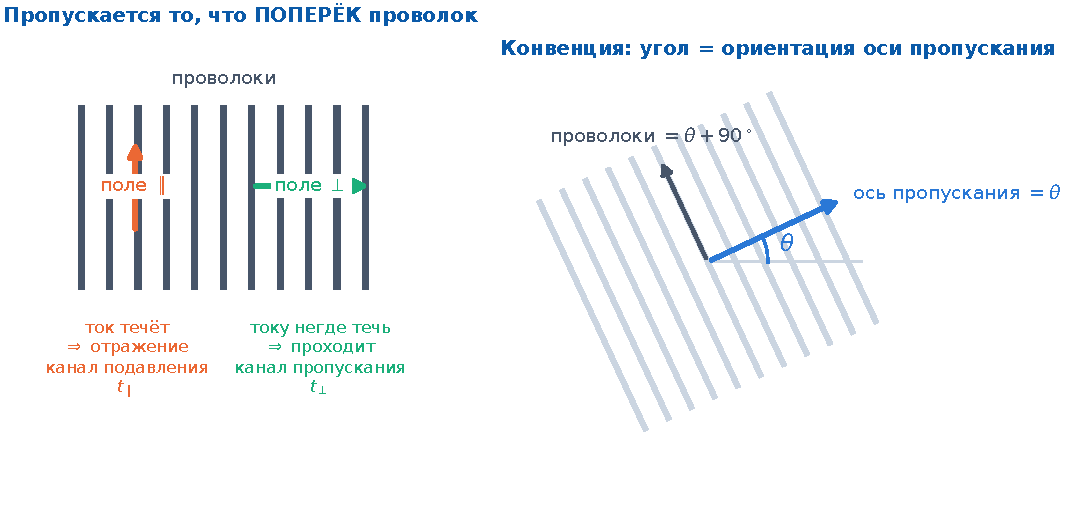
\includegraphics[width=\linewidth]{figures/fig00_geometry.pdf}
  \caption{Слева: два канала решётки. Справа: конвенция репозитория~--- угол элемента есть
  ориентация \emph{оси пропускания}, проволоки лежат под углом $\theta+90^\circ$
  (\artifact{research/two\_wgp/model\_2wgp.py}).}
  \label{fig:geometry}
\end{figure}

\needspace{8\baselineskip}   % не давать рисунку разорвать эту врезку
\begin{warning}[: здесь ошибаются почти все]
Проволочная решётка~--- \textbf{не щель}. Интуиция «щель в заборе пропускает то, что вдоль щели»
даёт \emph{противоположный} ответ. Правильно: \textbf{поляризатор пропускает поле, перпендикулярное
проволокам.} Ошибка стоит поворота всех углов на~$90^\circ$ и переворачивает физический смысл
каждого результата.
\end{warning}

\noindent
Отсюда \term{конвенция репозитория}: угол элемента~--- ориентация \emph{оси пропускания}
(перпендикуляра к проволокам), сами проволоки лежат под углом $+90^\circ$ к ней. Читая в проекте
«угол~$\theta$», подставляйте «ось пропускания», а не «проволоки».

\begin{strict}
В собственных осях решётки её действие~--- диагональная матрица
\[
  J_{\text{решётка}}=\begin{pmatrix}\tperp(\nu) & 0\\[2pt] 0 & \tpar(\nu)\end{pmatrix},
\]
то есть вся электродинамика решётки сводится к \emph{двум комплексным числам на каждой частоте}.
Откуда эти числа берутся аналитически~--- \S2 (модель Бланко); какие материальные поправки к ним
добавляются~--- \S3 (Друде и рассеяние~$\nu^\gamma$).
\end{strict}

% ---------------------------------------------------------------------
\subsection{Подволновой режим: почему решётка «сплошная»}

\paragraph{Вопрос.} Решётка~--- периодическая структура с промежутками. Почему она описывается
двумя числами, а не картиной дифракции на каждой проволоке?

\begin{intuition}[: ответ в соотношении масштабов]
Рабочий диапазон проекта $0.2\ldots1.5$~ТГц, период решёток $P=15\ldots40$~мкм, то есть
$\lambda=200\ldots1500$~мкм и $P/\lambda\lesssim0.2$. Волна на порядок-два длиннее периода и
физически не разрешает отдельные проволоки~--- так же, как длинная океанская волна не «видит»
отдельных свай пирса, а чувствует пирс целиком (рис.~\ref{fig:scales}).
\end{intuition}

\begin{figure}[t]
  \centering
  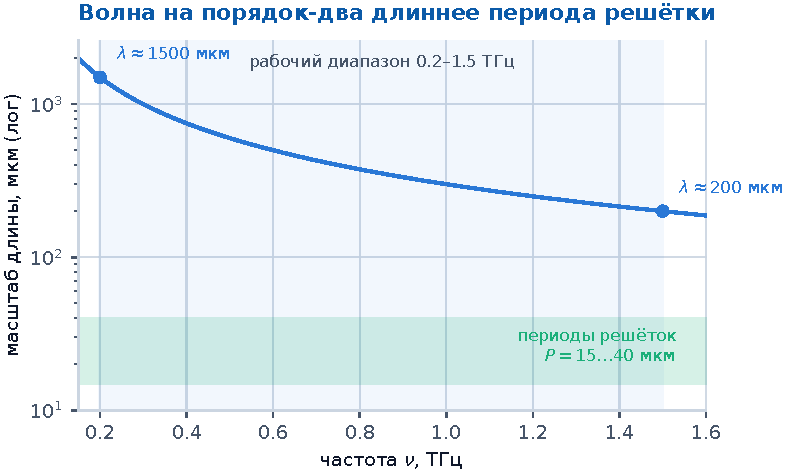
\includegraphics[width=0.78\linewidth]{figures/fig00_scales.pdf}
  \caption{Длина волны во всём рабочем диапазоне на порядок-два превышает период решёток проекта.
  Отсюда подволновой режим и законность описания решётки эффективным листом.}
  \label{fig:scales}
\end{figure}

\begin{strict}[: дифракционные порядки]
Решётка с периодом~$P$ рассеивает волну в порядки с поперечным волновым числом
$k_x^{(m)}=k\sin\alpha_{\text{пад}}+2\pi m/P$. Порядок распространяется, только если
$|k_x^{(m)}|\le k=2\pi/\lambda$, то есть требуется $P\gtrsim\lambda$. При $P\ll\lambda$ все порядки
$m\neq0$ имеют $|k_x^{(m)}|>k$, продольное волновое число $k_z=\sqrt{k^2-k_x^2}$ становится
\emph{мнимым}, и такие волны \term{эванесцентны}: экспоненциально затухают от решётки и энергию не
уносят.

\textbf{Следствие.} В дальнее поле уходит только нулевой порядок. Наблюдаемая~--- одно прошедшее
поле, а не набор пучков, и структура законно заменяется эффективным анизотропным листом с двумя
коэффициентами $\tperp,\tpar$. Именно это оправдывает весь формализм Джонса в проекте.
\end{strict}

\begin{projectfact}[: тот же объект в другом диапазоне~--- обычная решётка]
Период образца \texttt{purewave} независимо измерен по дифракции лазерной указки:
$P=23.4\pm0.8$~мкм~--- согласуется с микрофотографией $25.5\pm0.9$~мкм в пределах $1.8\sigma$
(Сессия~A, задача~A8; \artifact{coordination/BOARD.md}, запись от 2026-08-04).

Обратите внимание: дифракционные порядки \emph{видимого} света на этой решётке прекрасно
наблюдаются ($\lambda\approx0.65$~мкм $\ll P$). Подволновой режим~--- свойство не решётки, а
\emph{пары} «решётка~+~длина волны».
\end{projectfact}

% ---------------------------------------------------------------------
\subsection{Параметр плотности $D/P$}

\begin{intuition}
$D$~--- диаметр проволоки, $P$~--- период (расстояние между осями соседних проволок). Безразмерное
отношение $D/P$~--- доля периода, занятая металлом. В подволновом режиме абсолютные размеры сами по
себе не важны: важны их отношения к $\lambda$ и друг к другу. Именно $D/P$ управляет тем, насколько
плотно решётка «замыкает» тёмный канал.
\end{intuition}

\begin{figure}[t]
  \centering
  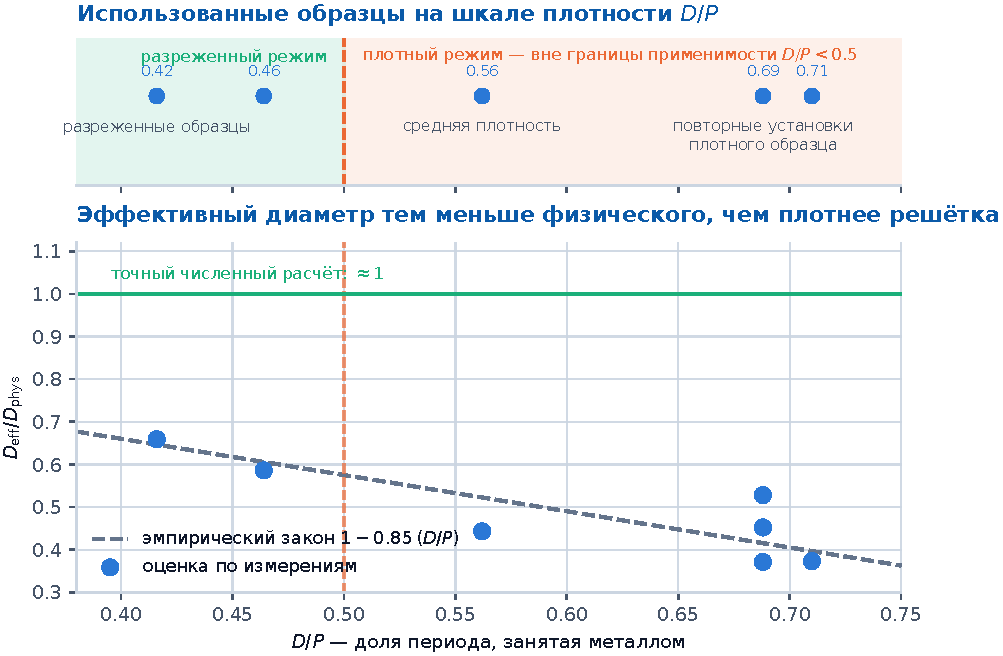
\includegraphics[width=0.86\linewidth]{figures/fig00_dp.pdf}
  \caption{Вверху: положение семи наборов проекта на шкале плотности и граница применимости
  аналитики, объявленная самим Бланко ($d/p<0.5$). Внизу: дефицит эффективного диаметра против
  плотности вместе с эмпирическим законом $1-0.85\,(D/P)$ и результатом точного расчёта. Числа~---
  \artifact{BRIEF\_FOR\_D\_teaching\_ladder.md} §11.3, колонка полного углового диапазона.}
  \label{fig:dp}
\end{figure}

\noindent
Практически все различия между образцами в проекте выстраиваются именно по $D/P$~--- не по
производителю и не по дате съёмки (рис.~\ref{fig:dp}):

\begin{itemize}[leftmargin=1.4em,itemsep=0.25em]
  \item \textbf{утечка тёмного канала:} $\eta\approx0.012$ при $D/P=0.71$ против $\approx0.033$ при
        $D/P=0.46$~--- более плотная решётка течёт \emph{слабее}, то есть является лучшим
        поляризатором (знак физически верен, \artifact{research/SYNTHESIS.md} §2);
  \item \textbf{применимость аналитики:} сам Бланко объявил границу $d/p<0.5$~--- плотные образцы
        проекта лежат \emph{вне} паспорта модели (находка Сессии~L,
        \artifact{research/papers/litrev/answers/}; подробно в~\S2);
  \item \textbf{дефицит эффективного диаметра} $\Deff/\Dphys$ монотонно падает от $0.659$ при
        $D/P=0.416$ до $0.373$ при $D/P=0.710$, тогда как точный расчёт даёт $\approx1$. Это
        центральная открытая загадка проекта, и разбирается она в~\S6 и~\S9.
\end{itemize}

\begin{warning}[: терминология, обязательная и в статье]
Четыре набора \texttt{att-11-16-*}~--- это \textbf{не четыре образца}, а ОДИН прибор
(ATT-11-16-CA85, S/N~\#02721) в четырёх условиях съёмки
(\artifact{BRIEF\_FOR\_D\_teaching\_ladder.md} §11.4). Называть их четырьмя образцами~--- значит
вчетверо завысить объём выборки.
\end{warning}

% ---------------------------------------------------------------------
\subsection{Честная оговорка: пучок конечной ширины}

Всё изложенное выше молча предполагало \term{плоскую волну}~--- бесконечно широкий фронт и один
угол падения. Реальный эксперимент устроен не так, и об этом следует сказать прямо (в статье это
идёт в раздел ограничений).

\begin{projectfact}[: сколько длин волн укладывается в пучок]
Пучок в перетяжке имеет диаметр $1.5\ldots2$~мм (\artifact{data\_pool/purewave/README.md}, раздел
про оптическую схему). При $\lambda=200\ldots1500$~мкм это всего \textbf{1--10 длин волн}.
\end{projectfact}

\noindent
Отсюда три следствия:
\begin{enumerate}[leftmargin=1.6em,itemsep=0.3em]
  \item \textbf{«Угол падения»~--- не одно число.} Сфокусированный пучок есть суперпозиция плоских
        волн с разными направлениями (широкий угловой спектр), тогда как аналитическая модель
        считает нормальное падение одной плоской волны.
  \item \textbf{Пространственное разрешение частотно-зависимо.} Низкие частоты «размазаны» шире
        высоких, то есть разные частоты опрашивают \emph{разные участки} образца.
  \item \textbf{Реальный кейс, стоивший проекту отозванного вывода.} Поляризатор в перетяжке был
        намеренно смещён относительно оси вращения. Узкий пучок при повороте образца описывает по
        апертуре окружность~--- следовательно, \emph{угол и участок образца перепутаны}. Вывод по
        гипотезе HN15 («дефицит $\Deff$ растёт с нерегулярностью решётки») был опубликован утром и
        отозван тем же вечером после уточнения схемы владельцем; текущий статус HN15~---
        \textbf{НЕ ПРОВЕРЕНА} (\artifact{BRIEF\_FOR\_D\_teaching\_ladder.md} §11.2).
\end{enumerate}

\begin{warning}[: правило, которое стоит запомнить раньше всей математики]
Прежде чем интерпретировать угловую развёртку, убедитесь, что образец отцентрован на оси вращения.
Иначе пространственная неоднородность образца подмешивается в $U(\theta)$~--- и, в отличие от
честной физики поляризатора, она \emph{не обязана быть чётной по}~$\theta$. Это, кстати,
действующий кандидат-объяснение асимметрии, отвергшей гипотезу~HN13 ($9.3\sigma$ / $4.2\sigma$;
не проверено).
\end{warning}

% ---------------------------------------------------------------------
\subsection{Типичные ошибки этого параграфа}

\begin{enumerate}[leftmargin=1.6em,itemsep=0.25em]
  \item Считать, что решётка пропускает поле \emph{вдоль} проволок. Наоборот
        (\S\ref{subsec:grid}).
  \item Путать угол оси пропускания с углом проволок. В коде проекта угол~--- ось пропускания.
  \item Переносить интенсивностную интуицию на THz-TDS. Детектор меряет \emph{поле}
        (\S\ref{subsec:field-vs-intensity}); отсюда пять, а не три независимых числа, и отсюда же
        вообще существует наблюдаемая~$\tleak$.
  \item Считать фазу технической деталью. Наклон фазы по частоте~--- это время
        (\S\ref{subsec:phase}), и оно измерено дважды независимо.
  \item Забывать про подволновость. Формализм $2\times2$ законен именно потому, что $P\ll\lambda$;
        на видимом свете тот же образец~--- обычная дифракционная решётка.
  \item Оперировать абсолютными микронами вместо~$D/P$: в подволновом режиме физику определяют
        безразмерные отношения.
  \item Молча предполагать плоскую волну. Пучок шириной 1--10 длин волн~--- это, помимо прочего,
        готовый механизм смешивания угла с координатой на образце.
\end{enumerate}

% ---------------------------------------------------------------------
\subsection*{Источники фактуры параграфа}
\addcontentsline{toc}{subsection}{\quad Источники фактуры §0}

\begin{center}
\footnotesize
\setlength{\tabcolsep}{4pt}
\begin{tabular}{@{}p{0.44\linewidth}>{\raggedright\arraybackslash}p{0.52\linewidth}@{}}
\toprule
\textbf{Утверждение} & \textbf{Артефакт} \\
\midrule
Данные~--- поле, не интенсивность & \texttt{CLAUDE.md} «Данные»; \texttt{data\_pool/**} \\
Пятимерный гармонический базис, невязка $1.4\times10^{-16}$ & \texttt{research/two\_wgp/NOTE\_malus\_linearization.md}; \texttt{results/two\_wgp/a0\_malus\_linearization.json} \\
$A_4/A_2$ по образцам ($0.2458\ldots0.2549$) & \texttt{BRIEF\_FOR\_D\_teaching\_ladder.md} §5.2 \\
$\tleak=0.19$~пс, сдвиг пика $-0.31$~пс & \texttt{research/SYNTHESIS.md} (HN8) \\
Конвенция угла = ось пропускания & \texttt{research/two\_wgp/model\_2wgp.py} \\
Период по дифракции $23.4\pm0.8$ против микрофото $25.5\pm0.9$~мкм & Сессия~A, A8; \texttt{coordination/BOARD.md} (2026-08-04) \\
Таблица $D/P$ и $\Deff/\Dphys$ по семи наборам & \texttt{BRIEF\_FOR\_D\_teaching\_ladder.md} §11.3 \\
Граница применимости Бланко $d/p<0.5$ & \texttt{research/papers/litrev/answers/} (Сессия~L, P1) \\
Пучок 1.5--2~мм, смешивание угла с участком, статус HN15 & \texttt{data\_pool/purewave/README.md}; \texttt{BRIEF\_FOR\_D\_teaching\_ladder.md} §11.2 \\
\bottomrule
\end{tabular}
\end{center}

\clearpage
